%%%%%%%%%%%%%%%%%%%%%%%%%%%%%%%%%%%%%%%%%
% Short Sectioned Assignment
% LaTeX Template
% Version 1.0 (5/5/12)
%
% This template has been downloaded from:
% http://www.LaTeXTemplates.com
%
% Original author:
% Frits Wenneker (http://www.howtotex.com)
%
% License:
% CC BY-NC-SA 3.0 (http://creativecommons.org/licenses/by-nc-sa/3.0/)
%
%%%%%%%%%%%%%%%%%%%%%%%%%%%%%%%%%%%%%%%%%

%----------------------------------------------------------------------------------------
%	PACKAGES AND OTHER DOCUMENT CONFIGURATIONS
%----------------------------------------------------------------------------------------

\documentclass[paper=a4, fontsize=11pt]{scrartcl} % A4 paper and 11pt font size
\usepackage[UTF8]{ctex}%Use Chinese charactors.
\usepackage[T1]{fontenc} % Use 8-bit encoding that has 256 glyphs
\usepackage{fourier} % Use the Adobe Utopia font for the document - comment this line to return to the LaTeX default
\usepackage[english]{babel} % English language/hyphenation
\usepackage{amsmath,amsfonts,amsthm} % Math packages
\usepackage{graphicx}
\usepackage{xcolor}
\usepackage{titlesec} %Used for title setting
\usepackage{listings} %Use code

\usepackage{lipsum} % Used for inserting dummy 'Lorem ipsum' text into the template

\usepackage{sectsty} % Allows customizing section commands
%\allsectionsfont{\Large} % Make all sections centered, the default font and small caps
%\allsectionsfont{\centering \normalfont\scshape} % Make all sections centered, the default font and small caps

\usepackage{fancyhdr} % Custom headers and footers
\pagestyle{fancyplain} % Makes all pages in the document conform to the custom headers and footers
\fancyhead{} % No page header - if you want one, create it in the same way as the footers below
\fancyfoot[L]{} % Empty left footer
\fancyfoot[C]{} % Empty center footer
\fancyfoot[R]{\thepage} % Page numbering for right footer
\renewcommand{\headrulewidth}{0pt} % Remove header underlines
\renewcommand{\footrulewidth}{0pt} % Remove footer underlines
\setlength{\headheight}{13.6pt} % Customize the height of the header


\numberwithin{equation}{section} % Number equations within sections (i.e. 1.1, 1.2, 2.1, 2.2 instead of 1, 2, 3, 4)
\numberwithin{figure}{section} % Number figures within sections (i.e. 1.1, 1.2, 2.1, 2.2 instead of 1, 2, 3, 4)
\numberwithin{table}{section} % Number tables within sections (i.e. 1.1, 1.2, 2.1, 2.2 instead of 1, 2, 3, 4)

\setlength\parindent{0pt} % Removes all indentation from paragraphs - comment this line for an assignment with lots of text

%----------------------------------------------------------------------------------------
%	TITLE SECTION
%----------------------------------------------------------------------------------------

\newcommand{\horrule}[1]{\rule{\linewidth}{#1}} % Create horizontal rule command with 1 argument of height

\title{	
\normalfont \normalsize
\textsc{Report} \\ [25pt] % Your university, school and/or department name(s)
\horrule{0.5pt} \\[0.4cm] % Thin top horizontal rule
\huge Weekly Report \\ % The assignment title
\horrule{2pt} \\[0.5cm] % Thick bottom horizontal rule
}

\author{Li Yuhang} % Your name

\date{\normalsize\today} % Today's date or a custom date
\begin{document}

\maketitle % Print the title
%----------------------------------------------------------------------------------------
This document is daily reports of my paper on model registration. It records my work on the project day by day. And it will be updated every day.

\section{2016-10-8}
\subsection{ICP algorithm test}
I found and tested a source code of the ICP algorithm on a point cloud. I firstly transformed the initial point cloud (white in Fig~\ref{icp_fish}) to get a transformed point cloud (green in Fig~\ref{icp_fish}) with a randomly selected Rotation Matrix $\textbf{R}$ and a Translation Matrix $\textbf{T}$. And then I used the ICP algorithm to compute $\textbf{R}$ and $\textbf{T}$. The red point cloud shows the aligned point cloud after transforming using the resultant rotation and translation matrix.

Fig~\ref{icp_fish} also shows both the input and the resultant parameters. 

\subsection{Plan of tomorrow} I will try to test it with my data. But before that I have to find a proper corner detection algorithm and to find a proper definition of 3D feature points. 
\begin{figure}
	\label{icp_fish}
	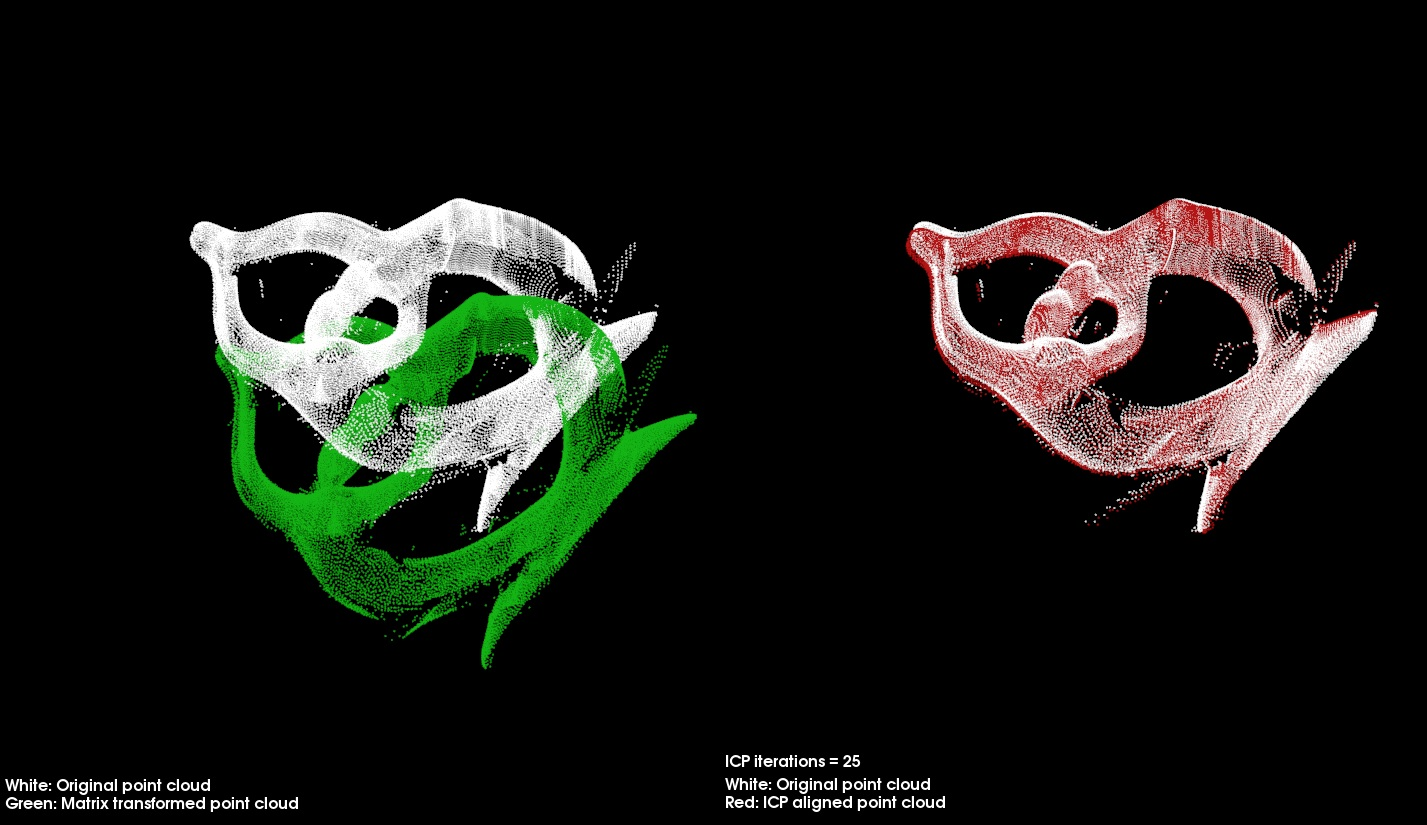
\includegraphics[width=\textwidth]{figures/2016-10-8/icp_result_fish}
	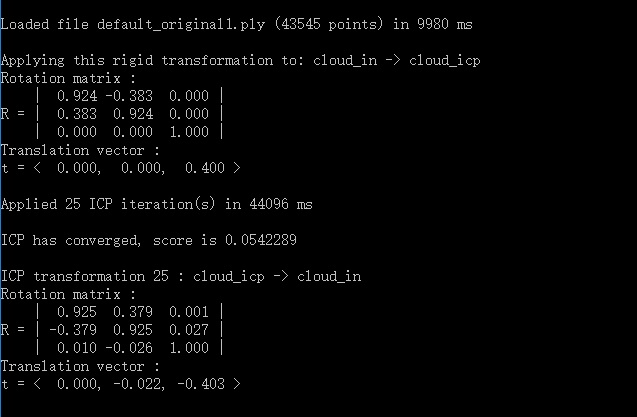
\includegraphics[width=\textwidth]{figures/2016-10-8/icp_result}
	\caption{The results of registration using ICP algorithm.}
\end{figure}
%----------------------------------------------------------------------------------------
%\bibliographystyle{plain}%
%\bibliography{F:/Hang/Report/Model_alignment/Bib/Alignment_of_Model}
\end{document}

